\documentclass[11pt]{article}
\usepackage{mypackages}
\begin{document}

\maketitle

\section{Deep learning}\label{sec:deep_learning}

In section \ref{sec:et} we mentioned that the state-value function and policy
can be estimated with a neural network.
The network can be seen as a function $f^\sim(x, w)$ that approximates a
function $f(x)$.
The parameters of the network, $w$, can be updated in many different ways, and in
this project we will update them based on the schemes described in section \ref{sec:a3c}
and \ref{sec:actor_critic}.

\subsection{Layers, neurons and connections}\label{sec:lnc}

To approximate $f(x)$ the network uses a combination of simpler functions.
More formally, a neural network consists of a number of \textit{layers},
that each represent a function $f^i : \R^{d} \to \R^k$, for a one dimensional layer.
This means the network can be seen as a composition of the functions
\begin{equation}
    f^\sim(x) = f^n(f^{n-1}( \cdots f^1(x) \cdots))
\end{equation}
for a network with $n$ layers.

The layers of the network inbetween the input and output layer, are called
\textit{hidden layers}, because we won't be directly seeing ther output
\cite{DeepLearningBook}.

Instead of trying to approximate the function $f^\sim(x)$ directly,
a neural network uses a lot of less complex functions.
The beginning of the network can then be pretty simple, but by the combination of the results of
the simpler functions, it is able to solve complex problems in the end.
We call this structure a hierarchy of concepts, where each concept can be described in terms
of the previous and simpler concepts\cite{DeepLearningBook}.
Each layer consists of a number of \textit{neurons} that are connected to the
neurons of the next layer
\begin{figure}[!h]
    \centering
    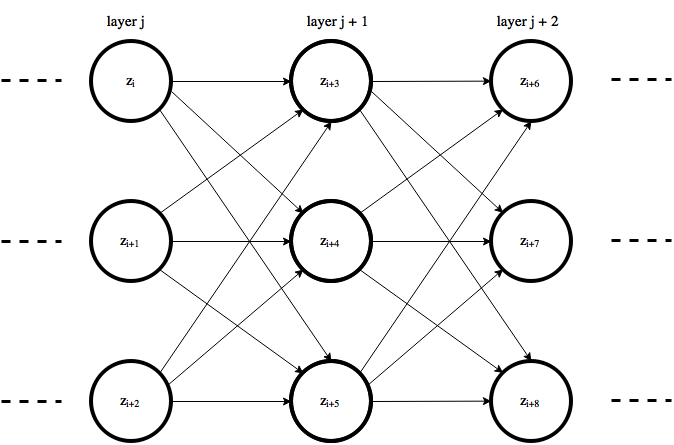
\includegraphics[width=10cm]{include/layers.png}
    \caption{A series of layers in a fully connected neural network.}
    \label{fig:layers}
\end{figure}

A neuron is a construct that transforms a series of input signals into a signle output signal.
Each of the input signals are sent through a \textit{weighted connection}, which means
that the input $a_i$ to neuron $z_i$ is given by
\begin{equation}
    a_i = \sum\limits_{j} w_{ij}* z_j
\end{equation}
for all neurons $z_j$ with a connection to $z_i$.

The purpose of each of the hidden layers is to extract some features from the input.
It does so by using an \textit{activation function}, $h : \R^d \to \R$, on the
weighted input it receives.
By combining the features extracted by the different hidden layers, the network
is trying to approximate $f(x)$.
The only way to change the network is by altering the weighted connections
between the neurons, and the general idea is to change the weights such that
$f^\sim(x)$ varies the least from $f(x)$ for all $x$.

%%%% A drawing of a neuron “up close”
\begin{figure}[!h]
    \centering
    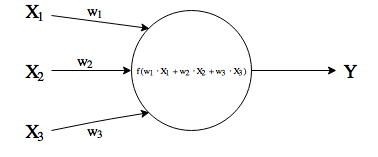
\includegraphics[width=10cm]{include/neuron.png}
    \caption{The structure of a single neuron with activation function $\alpha$.}
    \label{fig:neuron}
\end{figure}

The choice of activation function depends on the task the
network is supposed to solve.
E.g. when learning to play Atari games we want to estimate a policy,
that maximizes the expected return for each state.
To produce a probability distribution we can use the softmax function in the
final layer.
The softmax is defined as
\begin{equation}
    \text{softmax}(x) = \frac{exp(x_i)}{\sum\limits_{k=1}^K exp(x_k)}, \text{ for } i = 1, \dots, K
\end{equation}
for a $k$ dimensional input $x$ and is a generalization of the sigmoid function
shown below.
\begin{figure}[!h]
    \centering
    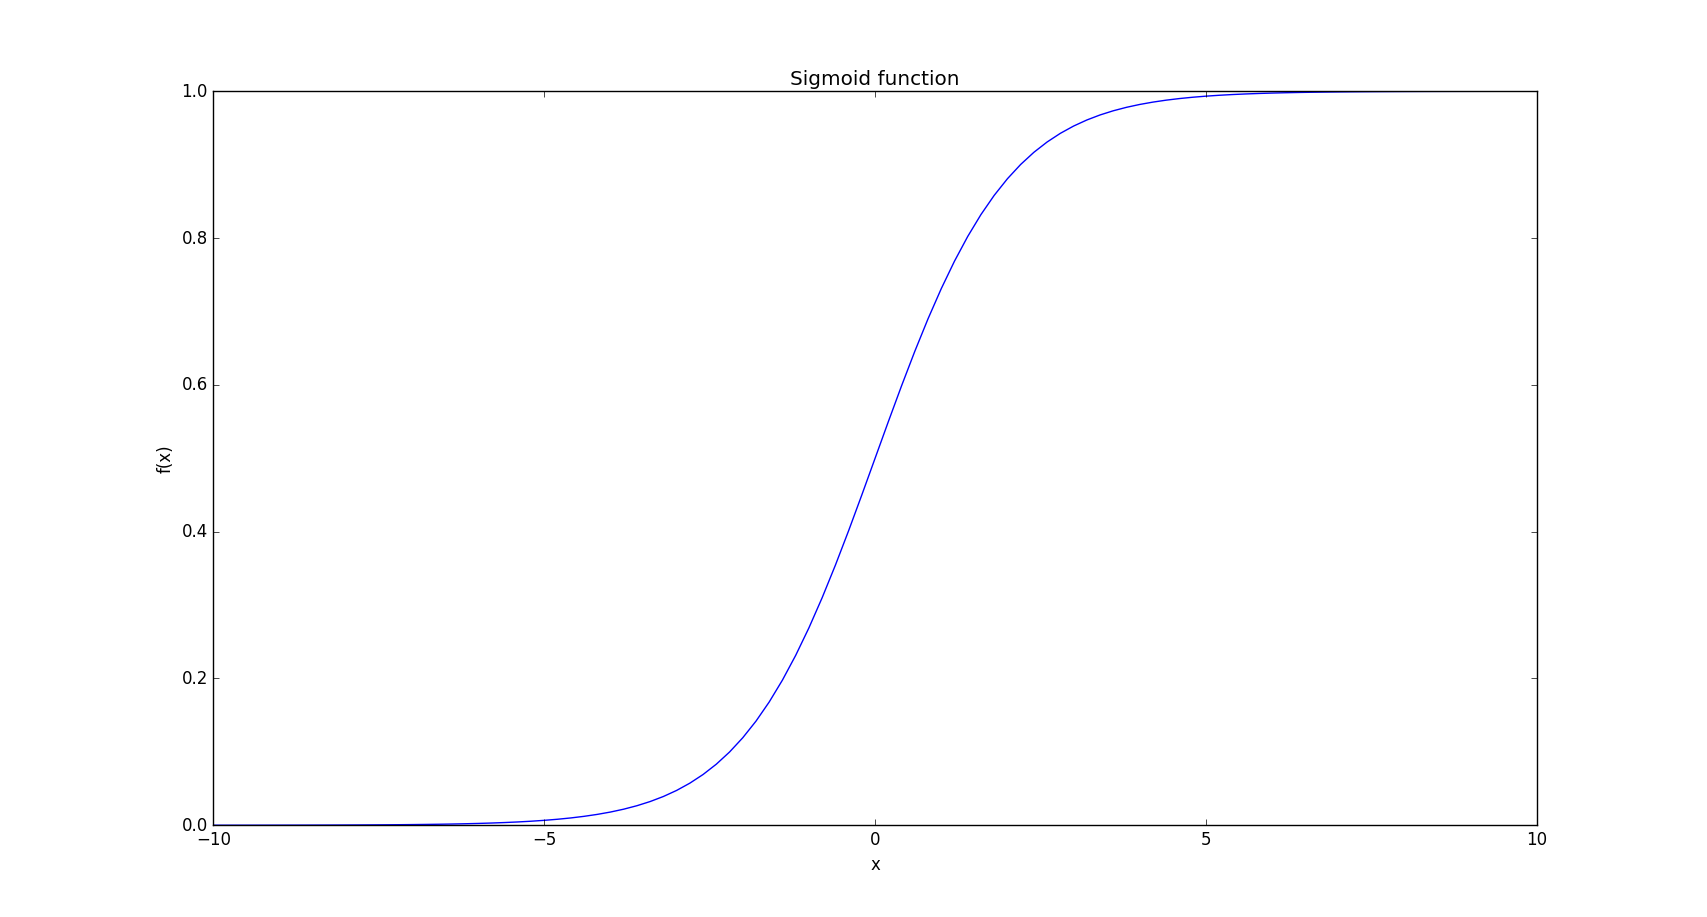
\includegraphics[width=15cm]{include/sigmoid.png}
    \caption{Plot of the sigmoid function.}
    \label{fig:softmax}
\end{figure}

The only other activation function we will be using in this project
is the \textit{rectified linear unit} (RELU), which is defined as
\begin{equation}
    f(x) = \max(0,x)
\end{equation}
This means that the all negative input values are changed to positive
values.

Thus, the role of the output of each layer is to provide some additional
transformation from the features in order to complete the task the network
must perform\cite{DeepLearningBook}.

\subsubsection{Learning from multidimensional input}

To process the high dimensional frames from the Atari games we will be using
a convolutional neural network (CNN).
A convolutional neural network typically performs three operations - a \textit{convolution},
a \textit{pooling} and an activation.

This means that the input to the CNN will be a two dimensional input with a single
channel. A convolution in two dimensions of a discrete image $I$ with filter kernel $K$
is given by 
\begin{equation}
    S(i, j) = (I \ast K)(i, j) = \sum\limits_m \sum\limits_n I(m, n) * K(i - m, j - n)
\end{equation}
where the kernel filter $K$ is a function $K : \R^{(d, k)} \to \R$.
A 2d convolutional layer takes advantage of the spatial structure in the input data to contruct a feature map
using the linear filter $K$.
A non-linear function is then applied to the feature map elements resulting from the convolution,
and the process as a whole can be seen as neurons with shared weights\cite{IgelConv}.

So in the network the kernel filter is the weights shared between the neurons of a
singe convolutional layer, which can be represented as a $d \times k$ dimensional matrix.
$$
K =
\begin{bmatrix}
    w_{1,1 } & w_{1, 2} & \hdots & w_{1, k} \\
    w_{2,1 } & w_{2, 2} & \hdots & w_{2, k} \\
    \vdots   &          & \ddots &          \\
    w_{d,1 } & w_{d, 2} & \hdots & w_{d, k} \\
\end{bmatrix}
$$
Each element in the resulting feature map descibres the weighted sum of its neighbouring
pixels, which means the result of a convolution can be seen as a feature exracted from
the input.
For a $4 \times 4$ input image and a $3 \times 3$ kernel filter the convolution
would be given by
%%% 2d convolution
\begin{figure}[!h]\label{conv2}
    \centering
    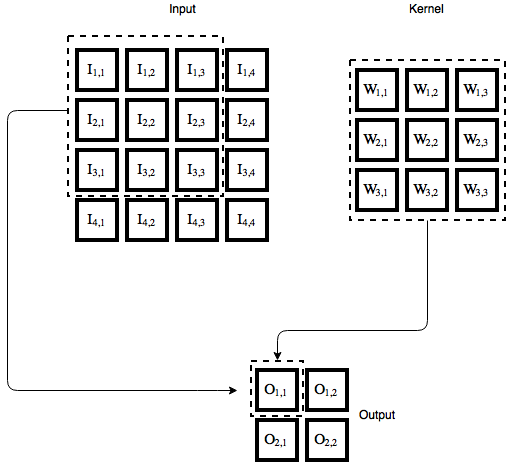
\includegraphics[width=10cm]{include/conv_2.png}
    \caption{A 2d convolution on an image which produces a \textit{feature} map.}
    \label{fig:conv}
\end{figure}
A problem with the convolution shown in figure \ref{conv2} is that
pixels at the boundary of the image are lost.
To deal with this issue we make use of zero padding.
By adding zeros to the border of each image, until the kernel
filter fits around each pixel, the image can maintain its dimensions, since the
padding is all that is lost now.
%%% Zero padded 2d convolution
\begin{figure}[!h]\label{con2}
    \centering
    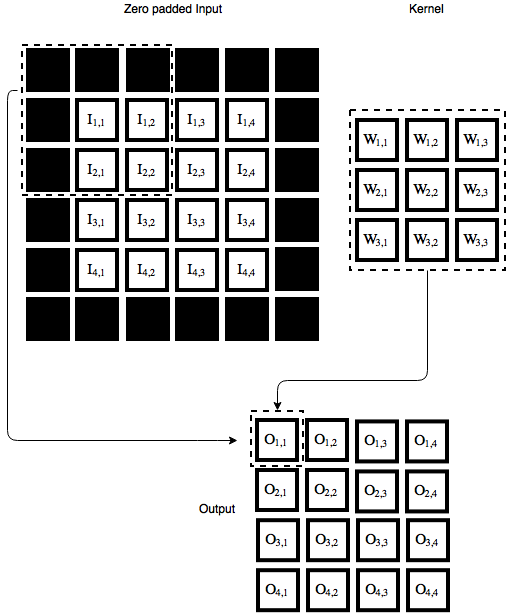
\includegraphics[width=10cm]{include/conv_2_zero_pad.png}
    \caption{The effect of zero padding the input image.}
    \label{fig:conv}
\end{figure}
The feature map consists of more separated objects than the original input,
which means we can more safely reduce the dimensionality without losing much information.
This reduction is called a pooling and is used to support
\textit{translation invariance}.
Translation invariance means that the features of the network should be able to
be extracted, regardless of their position in the feature map.
In an Atari game most objects move, while maintaining their original shape so being able to
extract information about objects independent of their position is very useful.

Instead of performing both a pooling and a convolutions in two separate steps,
we will be using convolutions \textit{with stride}.
This means we won't be applying the convolution to 
every element of the input, but instead every \textit{n'th} element,
%%%%% Strides
\begin{figure}[!h]\label{con2}
    \centering
    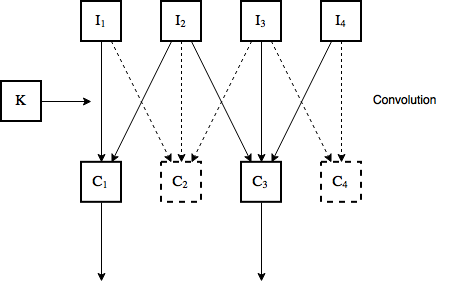
\includegraphics[width=10cm]{include/strides.png}
    \caption{A convolution in one dimension, using a stride of 2.
             This is effectively halving the size of the input, since
             the convolution is skipping every second element.}
    \label{fig:conv}
\end{figure}
Here the convolution skips every second element, resulting in a downsampling
of the input.
In two dimensions a convolution can be seen as the kernel moving across
an image, which means the stride is the amount of pixels the filter is moved.
Therefore the dimensions of an image can be halved by using a stride of $(2, 2)$, meaning
the stride is performed in both dimensions.

The pooling operation usually computes the maximum or average of a region of
a feature map, and using convolution with strides emulates
this behaviour since the convolution
is seen as a weighted sum of neighbouring pixels.


%%% Move this to after Policy Gradients
%\subsubsection{Updating the weights of the network}

%A neural network is trained to minimize its total loss based on its \textit{loss
%function}.
%A loss function $\mathcal{L} : \R^K \to \R$ is supposed to describe how close the
%predictions are to the true result.
%In the reinforcement learning setting it is often difficult to estimate the
%true result.
%E.g. for a policy aproximator $\pi^{\sim}(A_t | S_t)$ we want to use the knowledge
%of wether or not action $A_t$ was  chosen in state $S_t$ to determine
%whether the probability of taking $A_t$ should be increased or decreased to
%reduce the loss of the network.
%Therefore the weights of the connections in the network are typically updated
%in a direction in the weight space.
%This direction describes how the weights should be updated to increases the
%probability of repeating the action $A_t$ the most on future visits to
%state $S_t$\cite{RLbook}.
%To find the direction we would use the \textit{gradient} of the probability of
%taking the action actually taken, since it exactly describes how to increate
%this probability.
%
%Now, this would increase the chance of picking action $A_t$ in state $S_t$ again,
%but we really only want to pick actions again that lead to a good return.
%Therefore the probability is generally updated proportionally to the
%return, since the network will then learn to favor actions that provide
%the highest return.
%

\documentclass[11pt]{article}
\usepackage{mypackages}
\begin{document}


\subsection{Updating the weights of a network}

In section \ref{sec:actor_critic} and \ref{sec:a3c} we discussed different
approaches available to update the weights of the policy and value estimator.
These approaches are based on the directional values
expressed by the gradient of the estimator, or an error measure containing
the estimator.
Taking the gradient of a function $f : \R^n \to \R$ with respect to
some parameters $x \in \R^n$ is given by
\begin{equation}
    \nabla_x f(x)
    = \begin{pmatrix}
        \frac{\partial f(x)}{\partial x_1}\\
        \frac{\partial f(x)}{\partial x_2}\\
        \vdots\\
        \frac{\partial f(x)}{\partial x_n}
      \end{pmatrix}
\end{equation}

Now, in a neural network it is difficult to take the gradient of the
entire network at once, since it consists of a number of layers
using different activation functions and a lot of parameters.
To solve this issue the general approach to computing the gradient of a network
is to use \textit{back-propagation} as presented in \cite{IgelBackProp}
and \cite{DeepLearningBook}.

Consider a network consisting of $d$ input neurons, $M$ hidden neurons and $K$ output neurons,
estimating the function $f : \R^d \to \R^K$.
Each neuron can be denoted as $z_i$, where neurons for which $i \leq d$ are the input neurons, $d < i \leq M + d$ are the hiden neurons
and $M + d < i \leq M + d + K$ are the output neurons.
As described in section \ref{sec:lnc} each neuron $z_i$ can be seen as a weighted activation of its input.
For the neurons in the hidden layers and the output layer, this means $z_i = h(a_i)$, where 
$a_i = \sum_{j} w_{ij} * z_{j}$ is the weighted sum of the input to the i'th neuron and $h$ is an arbitrary
activation function.

Previously we updated the weights of an estimator with regards to some performance measure $\rho$ 
describing how well the policy and value functions are performing. 
Now, we want to find the directional changes for all weights in the network
in regards to the performance measure.
If all $h$ in the network are differentiable this results in the partial derivatives
\begin{equation}\label{part}
    \frac{\partial \rho}{\partial w_{ij}}
\end{equation}
describing the directional change for each weighted connection in the network from $z_j$ to $z_i$.

If we start by looking at this partial derivative in the $K$ output neurons of the
neural network, we can apply the chain rule of calculus to equation \ref{part},
\begin{equation}
    \frac{\partial \rho}{\partial w_{ij}} = \frac{\partial \rho}{\partial a_i} \frac{\partial a_i}{\partial w_{ij}} 
\end{equation}
since $w_{ij}$ is a part of $a_i$.
$\frac{\partial \rho}{\partial a_i}$ is denoted as $\delta_i$ and have that $\frac{\partial a_i}{\partial w_{ij}} = z_j$ since
$\frac{\partial a_i}{\partial w_{ij}} = \frac{\partial}{\partial w_{ij}} \sum_{d} w_{id} * z_d = z_j$.
This means
\begin{equation}\label{eq:der}
    \frac{\partial \rho}{\partial w_{ij}} = \delta_i * z_j  
\end{equation}
For each of the output units, $\delta_i$ can be found as
\begin{equation}
    \begin{aligned}
        \delta_i & = \frac{\partial \rho}{\partial a_i}\\
        & = \frac{\partial \rho}{\partial z_i} \frac{\partial z_i}{\partial a_i}\\
        & = h'(a_i) \frac{\partial \rho}{\partial z_i} 
    \end{aligned}
\end{equation}
since $\frac{\partial z_i}{\partial a_i} =  \frac{\partial}{\partial a_i} h(a_i) = h'(a_i)$.
Therefore the partial derivative of the performance measure with respect to a weight from
an output neuron can be found as
\begin{equation}
    \frac{\partial \rho}{\partial w_{ij}} = h'(a_i) \frac{\partial \rho}{\partial z_i} * z_j
\end{equation}
This only holds for the output neurons because their output isn't
used by any other neuron.
For the hidden neurons we have to take all subsequent neurons into account as
well, since their output is propagated forward through the network.
Thus,
\begin{equation}
    \delta_i = \sum\limits_{k=i+1}^{M + d + K} \frac{\partial \rho}{\partial a_k} \frac{\partial a_k}{\partial a_i} 
\end{equation}
for all hidden neurons, $z_i$, for which $d > i \leq M + d + K$.
Since $\frac{\partial \rho}{\partial a_k} = \delta_k$ and
$\frac{\partial a_k}{\partial a_i} = \frac{\partial a_k}{\partial z_i} \frac{\partial z_i}{\partial a_i}$ we
can derive $\delta_i$ as
\begin{equation}
    \begin{aligned}
        \delta_i & = \sum\limits_{k=i+1}^{M + d + K} \delta_k \frac{\partial a_k}{\partial z_i} \frac{\partial z_i}{\partial a_i}\\
        & = \sum\limits_{k=i+1}^{M + d + K} \delta_k * w_{ki} *  h'(a_i)\\
        & = h'(a_i) \sum\limits_{k=i+1}^{M + d + K} \delta_k * w_{ki}
    \end{aligned}
\end{equation}
because $\frac{\partial a_k}{\partial z_i} = \frac{\partial}{\partial z_i} \sum_{j} w_{kj} * z_j = w_{ki}$.
Using these equations, we can then compute the partial derivatives for all output and hidden neurons
by computing $\delta$, since we already have access to the value of $z_j$.
However, it is important to note that the partial derivatives have to be computed in the reverse order,
since each derivative in each neuron, $z_j$, is dependant of all derivatives of all later neurons $z_i$ for $j < i$.


%%%% AFSLUTNING %%%%

Now that we have an understanding of the underlying principles of Deep Reinforcement Learning, we can apply it to real problems.
We have presented a lot of theory in the last sections,
with most important aspects being the fundamentals of the Actor-Critic method and how eligibility have a stabilizing effect on learning,
as well as the idea of using asynchronous training to speed up the training process, and lastly
how Deep Learning can be used to estimate a policy and the state-value function

\end{document}

\end{document}
